\documentclass[11pt]{article}
\usepackage[utf8]{inputenc}	% Para caracteres en español
\usepackage{amsmath,amsthm,amsfonts,amssymb,amscd}
\usepackage{multirow,booktabs}
\usepackage[table]{xcolor}
\usepackage{fullpage}
\usepackage{lastpage}
\usepackage{enumitem}
\usepackage{fancyhdr}
\usepackage{mathrsfs}
\usepackage{wrapfig}
\usepackage{setspace}
\usepackage{url}
\usepackage{calc}
\usepackage{multicol}
\usepackage{cancel}
\usepackage[retainorgcmds]{IEEEtrantools}
\usepackage[margin=3cm]{geometry}
\usepackage{amsmath}
\newlength{\tabcont}
\setlength{\parindent}{0.0in}
\setlength{\parskip}{0.05in}
\usepackage{empheq}
\usepackage{framed}
\usepackage[most]{tcolorbox}
\usepackage{xcolor}
\colorlet{shadecolor}{orange!15}
\parindent 0in
\parskip 12pt
\geometry{margin=1in, headsep=0.25in}
\theoremstyle{definition}
\newtheorem{defn}{Definition}
\newtheorem{reg}{Rule}
\newtheorem{exer}{Exercise}
\newtheorem{note}{Note}

%\newif\ifnotes
%\newcommand{\h}[1]{\ifnotes{\textcolor{red}{#1}}\fi}
\newcommand{\h}[1]{\textcolor{red}{#1}}

\begin{document}
\setcounter{section}{8}
\title{Chapter 9 Review Notes}

\thispagestyle{empty}

\begin{center}
{\LARGE \bf Convexity of Differentiable Function Approximations}\\
\end{center}
\section{Convexity Reference}

\subsection{Definitions}

There are several definitions and properties of convexity which are useful for determining where functions are convex.

\textbf{Definition.} A function $f(x)$ is \textit{convex} on interval $I$ if $\forall x_1, x_2 \in I, \forall \in [0, 1]: f(t x_1 + (1-t)x_2) \leq tf(x_1) + (1-t)f(x_2)$. 

\textbf{First Derivative} Using the first derivative this becomes: $\forall x_1, x_2 \in I: f(x_1) \geq f(x_2) + f'(x_2)*(x_1 - x_2)$. In other words, the derivative cannot decrease on $I$. 

\textbf{Second Derivative} This also means that $\forall x \in I: f''(x) \geq 0$

\subsection{Compositions}

\textbf{Summation and Multiplication} Sums of convex functions are convex. Multiplication by a constant is convex, provided the constant is greater than 0.

\textbf{Composition} If $f$ and $g$ are convex, $g \circ f$ is convex on intervals where $g' \geq 0$, (ie where $g$ is monotonically increasing).

\begin{figure}[h!]
  \centering
  %\includegraphics[width=\linewidth]{figs/mlp2.png}
  %\includegraphics[height=6cm]{figs/mlp2.png}
  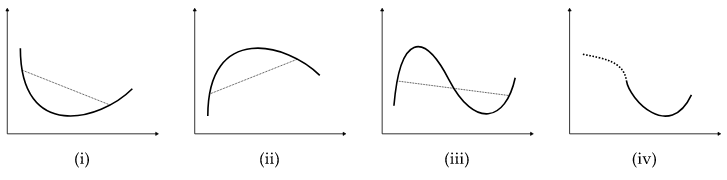
\includegraphics[width=\linewidth]{figs/convex_examples.png}
  \caption{Some examples of convex and concave functions. (from \protect\url{http://www.math.cmu.edu/~lohp/docs/math/mop2013/convexity-soln.pdf})}
  %\label{fig:mlp2}
\end{figure}

\section{Convexity of Integer Operations}
\subsection{Arithmetic Operations}

\textbf{Addition}. 
\begin{enumerate}
\item \textbf{Function:} $g(x) = x + c$ is trivially convex, since $g'(x) = 1$. , 
\item \textbf{Composition:}  $g \circ f$ is also convex given convex $f$, since $\forall x: g'(x) \geq 1$.
\item \textbf{Binary Composition:} For addition given two convex input functions $f_1$ and $f_2$: $g(f_1(x), f_2(x)) = f_1(x) + f_2(x)$. This is still convex, since $\frac{dg}{df_1} = \frac{dg}{df_2} = 1$. 
\item \textbf{Step size:} Step size does not affect convexity for additon ($Ax + b$ is an affine tranformation).
\end{enumerate}

\textbf{Subtraction}. 
\begin{enumerate}
\item \textbf{Function:} $g(x) = x - c$ is both trivially convex, since $g'(x) = 1$. , 
\item \textbf{Composition:}  $g \circ f$ is also convex given convex $f$, since $\forall x: g'(x) \geq 1$.
\item \textbf{Binary Composition:} This is still convex, since $\frac{dg}{df_1} = \frac{dg}{df_2} = 1$. For subtraction $g(f_1(x), f_2(x)) = f_1(x) - f_2(x)$, $g''(f_1(x), f_2(x)) = f_1''(x) - f_2''(x)$, this will be convex where $f_1''(x) \geq f_2''(x)$. For example, for $f_1(x) = x^2$, $f_2(x) = x^3$, $g(x)$ will be convex where the 2nd derivative $2 - 6x \geq 0$, ($x \leq \frac{1}{3}$).
\item \textbf{Binary Composition with bounds:} Given a particular interval $x \in I$ in which $f_1''(x) \in [d_{1low}, d_{1high}]$ and $f_2''(x) \in [d_{2low}, d_{2high}]$, $g(x)$ will be convex if $d_{1low} - d_{2high} \geq 0$, since this means $g''(x) \geq 0$ for $x \in I$.
\item \textbf{Step size:} Does not effect single function composition, for multiple function composition $x$ becomes $\frac{x}{s}$ (for step size $s$), which may effect the regions where $g(x)$ is convex depending on the input functions.
\end{enumerate}

\textbf{Multiplication}
\begin{enumerate}
\item \textbf{Function:} $g(x) = cx$  is trivially convex, since $g''(x) = 0$. , 
\item \textbf{Composition:}  $g \circ f$ is convex for convex $f$ when $c \geq 0$, since $g'(x) = c$. For concave $f$, the inverse holds. If $f''(x)$ is bounded, this simply means the lower bound must greater than 0 if $c>0$, or the upper bound must be less than 0 if $c<0$.
\item \textbf{Binary Composition:} For multiplication given two convex input functions $f_1$ and $f_2$: $g(f_1(x), f_2(x)) = f_1(x) * f_2(x)$. This is not convex in general, counterexample $g(-x, x) = -x^2$, but can be convex or convex in regions.
\item \textbf{Binary Composition with Bounds:} \h{Bounds don't seem to help much here, it seems you need more information about the functions. Example $g(x^2, -(x-2))$ is convex for $x<\frac{2}{3}$, how do you predict that from bounds on derivatives?}

\item \textbf{Step size:} $x = \frac{x}{s}$, does not effect single function composition.
\end{enumerate}


\textbf{Division}
\begin{enumerate}
\item \textbf{Function:} $g(x) = x/c$  is trivially convex, since $g''(x) = 0$. For $g(x) = c/x$, $g''(x) = 2cx^{-3}$, this is convex for $x \in [0, \inf), c \geq 0$, and $x \in (-\inf, 0), c < 0$. (note, may need to adjust this for integer division)
\item \textbf{Composition:} For $g(x) = x/c$, $g \circ f$ is convex when $c \geq 0$, since $g'(x) = c^{-1}$.  For $g(x) = c/x$, $g'(x) = -cx^{-2}$, then $\forall c < 0: g'(x) \geq 0$, and it is convex under composition for all $f(x)<0$. 
\item \textbf{Binary Composition:} Given two convex input functions $f_1$ and $f_2$: $g(f_1(x), f_2(x)) = f_1(x) / f_2(x)$. This is not convex in general, counterexample $g(x, x^2) = 1/x$, inputs are convex but output is concave, however it can still be convex or convex in regions.
\item \textbf{Binary Composition with Bounds:} \h{Similar issues to multiplication here.}
\item \textbf{Step size:} $x = \frac{x}{s}$, does not effect single function composition.
\end{enumerate}

\textbf{Exponentiation}
\begin{enumerate}
\item \textbf{Function:} $g(x) = x^c$  is convex if $c \mod 2 = 0$, since $g''(x) = (c-1)(c-2)x^{c-2} \geq 0$ if $c$ is even. If $c$ is odd, $g''(x) \geq 0$ for $x > 0$, so the function will be convex for $x>0$. ($x^1$ is the exception is convex everywhere).  For $g(x) = c^x$, it is convex for $c>0$ since $g''(x) = c^x \log^2(x)$. For $c<0$, the sign alternates so the function is convex over every interval $(x, x+2)$.

\item \textbf{Composition:} For $g(x) = x^c$, $g \circ f$ has second derivative $g''(x) = c(c-1) (f(x))^{c-2}f'(x) + cf(x)^{c-1}f''(x)'$. 
\item \textbf{Binary Composition:} For given two convex input functions $f_1$ and $f_2$: $g(f_1(x), f_2(x)) = f_1(x) ^ f_2(x)$. This does not preserve convexity in general, counterexample $g(-x, x) = -x^2$, inputs are convex but output is concave. 
\item \textbf{Step size:}  $x = \frac{x}{s}$, does not effect single function composition, where $g(x) = f(x)^c$, but renders analysis for $g(x) = c^{f(x)}$ invalid.
\end{enumerate}

\subsection{Bitwise Operations}

%\textbf{And}
\subsubsection*{And}
\begin{enumerate}
\item \textbf{Function:} For $g(x) = x \& c$, $g(x)$ will be convex in the following regions: let $k$ denote the number of contiguous leading bits in $c$ that share the same value, either 0 or 1. Then $g(x)$ will be convex where $x \in [x_k, x_k + 2^k - 1], x_k \mod 2^k = 0$. 

{\it Proof.} 

{\it Lemma 1} Only the first $k$ bits of $x$ change in the region $x \in [x_k, x_k + 2^k - 1] x_k \mod 2^k = 0$. Pf. The first $k$ bits of $x_k$ are 0 b/c $x_k \mod 2^k = 0$. Since the maximum in the region $x \in [x_k, x_k + 2^k - 1] x_k \mod 2^k = 0$ from $x_k$ is $2^k-1$, which is also represented in $k$ 1s, all changes in the region from $x_k$ only effect the first $k$ bits.

There are two cases, either the first $k$ bits are 0s or they are 1s. If they are 0s, then $g(x)$ will not change in the region $[x_k, x_k = 2^k-1]$ because from \textbf{lemma 1} only the first $k$ bits will change and the first $k$ bits are being bitwise $\&$ with $k$ 0s. Then $g(x) = g(x_k)$ in the region, and the definition of convexity applies. If the first $k$ bits are 1s, then from \textbf{lemma 1} any change in $x$ is anded with 1s, and $g(x) = g(x_k) + x - x_k$, which is linear and therefore a convex function.

Also note that for leading 1s, in some places the convexity region can be extended to include $x_k-1$: $x \in [x_k - 1, x_k + 2^k - 1] x_k \mod 2^k = 0$, while for the leading 0s, in some places the upper bound could be extended to $x_k + 2^k$. However these cases do not apply to all regions.

\item \textbf{Composition:} For $g \circ f$, the previous analysis holds when the leading bits are 0s for $f(x) \in [f(x)_k, f(x)_k + 2^k - 1] f(x)_k \mod 2^k = 0$, since $g(x)$ will still be constant in those regions. If the leading bits are 1s, then $g(x)$ is equivalent to multiplication by $1$ of $-1$, and convexity will be preserved if $f''(x) > 0$, or inverted if $f''(x) < 0$.
\item \textbf{Output bounds:} For leading 1s, bounds are limited to bounds in the convex region defined by the bitwise operation, or could remain the same if evaluating the input 2nd derivative in the region for tighter bounds is not feasible. For leading 0s, the 2nd derivative is set to 0 within the flat (convex) intervals.
\item \textbf{Step size:} If $s < 2^k$, then step size shrinks the convexity bounds to $\frac{2^k}{s}$, for $s > 2^k$, the input will jump between convex regions on changes in $x$. 
\end{enumerate}

\textbf{Composition} If $f$ and $g$ are convex, $g \circ f$ is convex on intervals where $g' \geq 0$, (ie where $g$ is monotonically increasing).

\begin{figure}[h!]
  \centering
  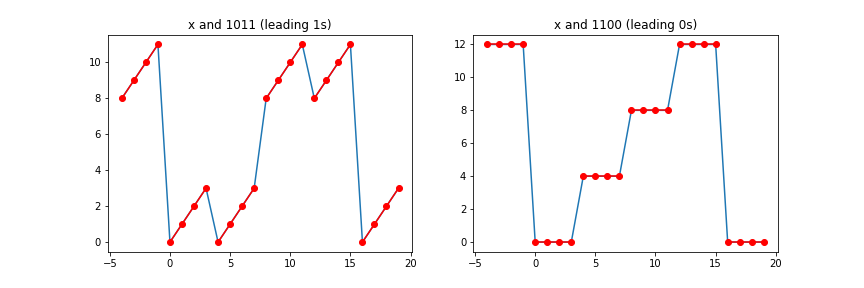
\includegraphics[width=\linewidth]{figs/and.png}
  \caption{Convex regions for bitwise \textbf{and}}
\end{figure}

%\textbf{Or}
\subsubsection*{Or}
\begin{enumerate}
\item \textbf{Function:}  For $g(x) = x | c$, $g(x)$ will be convex in the following regions: let $k$ denote the number of contiguous leading bits in $c$ that share the same value, either 0 or 1. Then $g(x)$ will be convex where $x \in [x_k, x_k + 2^k - 1], x_k \mod 2^k = 0$. 

{\it Proof.} There are two cases, either the first $k$ bits are 0s or they are 1s. If they are 1s, then $g(x)$ will not change in the region $[x_k, x_k = 2^k-1]$ because from \textbf{lemma 1} only the first $k$ bits will change and the first $k$ bits are being bitwise $|$ with $k$ 1s, setting them all to 1. Then $g(x) = g(x_k)$ in the region, and the definition of convexity applies. If the first $k$ bits are 0s, then from \textbf{lemma 1} any change in $x$ is bitwise \textbf{or}ed with 1s, and $g(x) = g(x_k) + x - x_k$, which is linear and therefore a convex function. 

\item \textbf{Composition:} For $g \circ f$, the previous analysis holds when the leading bits are 1s for $f(x) \in [f(x)_k, f(x)_k + 2^k - 1] f(x)_k \mod 2^k = 0$, since $g(x)$ will still be constant in those regions. If the leading bits are 0s, then $g(x)$ is equivalent to multiplication by $1$ of $-1$, and convexity will be preserved if $c > 0$, or inverted if $c < 0$. 
\item \textbf{Step size:} If $s < 2^k$, then step size shrinks the convexity bounds to $\frac{2^k}{s}$, for $s > 2^k$, the input will jump between convex regions on changes in $x$. 
\item \textbf{Output bounds:} For leading 0s, bounds are limited to bounds in the convex region defined by the bitwise operation, or could remain the same if evaluating the input 2nd derivative in the region for tighter bounds is not feasible. For leading 1s, the 2nd derivative is set to 0 within the flat (convex) intervals.
\end{enumerate}

\begin{figure}[h!]
  \centering
  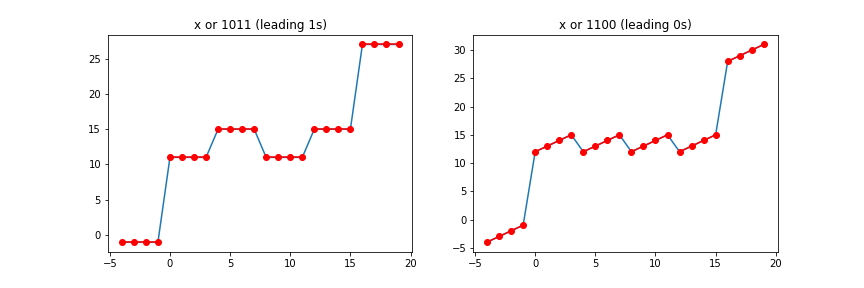
\includegraphics[width=\linewidth]{figs/or.png}
  \caption{Convex regions for bitwise \textbf{or}}
\end{figure}


%\textbf{Not}
\subsubsection*{Not}
\begin{enumerate}
\item \textbf{Function:} For $g(x) = ~x$, this is equivalent to $g(x) = -x - 1$, and as a linear function is convex. 
\item \textbf{Composition:} For $g \circ f$, $f$ will be inverted so that concave regions become convex. 
\end{enumerate}

%\textbf{Xor}
\subsubsection*{Xor}
\begin{enumerate}
\item \textbf{Function:} For $g(x) = x \oplus c$, $g(x)$ will be convex in the following regions: let $k$ denote the number of contiguous leading bits in $c$ that share the same value, either 0 or 1. Then $g(x)$ will be convex where $x \in [x_k, x_k + 2^k - 1], x_k \mod 2^k = 0$. 

{\it Proof.} There are two cases, either the first $k$ bits are 0s or they are 1s. If they are 0s, then $g(x) = g(x_k) + x - x_k$  in the region $[x_k, x_k = 2^k-1]$ because from \textbf{lemma 1} only the first $k$ bits will change and the first $k$ bits are being bitwise $\oplus$ with $k$ 0s, leaving them unchanged, and the definition of convexity applies. If the first $k$ bits are 1s, then from \textbf{lemma 1} any change in $x$ is bitwise $\oplus$ed with 1s, and $g(x) = g(x_k) - x + x_k$, which is also linear and therefore a convex function. 
\item \textbf{Composition:} For $g \circ f$, $f$ will be unchanged in the convex regions if there are leading 0s, preserving convexity in these regions, or inverted if there are leading 1s, making any concave parts of the function convex.
\item \textbf{Step size:} If $s < 2^k$, then step size shrinks the convexity bounds to $\frac{2^k}{s}$, for $s > 2^k$, the input will jump between convex regions on changes in $x$. 
\item \textbf{Output bounds:} For leading 1s, bounds are inverted in the convex region defined by the bitwise operation. For leading 1s, bounds remain the same, or could be tightened to the range within the convex region of the xor.
\end{enumerate}


\begin{figure}[h!]
  \centering
  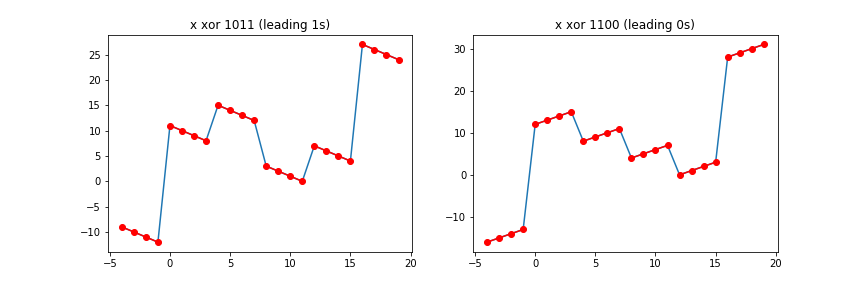
\includegraphics[width=\linewidth]{figs/xor.png}
  \caption{Convex regions for bitwise \textbf{xor}}
\end{figure}
%\begin{figure}
  %\centering
%\begin{subfigure}{.5\textwidth}
  %\centering
  %%\includegraphics[width=\linewidth]{figs/mlp2.png}
  %\includegraphics[height=6cm]{figs/mlp2.png}
  %\caption{Multilayer Perceptron with 2 hidden layers.}
%\end{subfigure}%
%\begin{subfigure}{.5\textwidth}
  %\centering
  %\includegraphics[height=6.5cm]{figs/mlp3.png}
  %\caption{Multilayer Perceptron with 2 hidden layers and residual connections.}
%\end{subfigure}
  %\caption{Two Layer MLPs.}
  %\label{fig:mlp2}
%\end{figure}

\end{document}
